\chapter{Background and Related Work}
\label{cha:background}

This chapter will introduce a concept of containerization, orchestration along with exploring fundamental concepts of Kubernetes tool, addressing the management of incoming (ingress) and outgoing (egress) traffic within a Kubernetes cluster. Finally, comparation of selected Container Network Interface plugins, pointing out their key features. The end will conclude with a literature overview.


%---------------------------------------------------------------------------
\section{Basics}
\label{sec:basics}

In this section two key Kubernetes concepts will be outlined.

\subsection{Containerization}
\label{sec:containerization}

Containerization is packaging an app along with all necessary runtime stuff like libraries, executables or assets into an object called "container". The main benefits of container are\cite{RedhatContainerization}: 

\begin{itemize} 
    \item Protable and Flexible -- container can be run on bare metal or virtual machine in cloud regardless of operating system. Only container runtime software like Docker Engine or containerd is required, which allows to interact with the host system. 

    \item Lightweight -- container is sharing operating system kernel with host machine, there is no need to install separate operating system inside 

    \item Isolated -- does not depends on host's environment or infrastructure 

    \item Standarized -- Open Container Initiative standardize runtime, image and distribution specifications 

\end{itemize} 

A container image is a set of files and configuration needed to run a container. It is immutable, only new images can be created with new changes. Consists of layers. The layer contains one modification made to an image. All layers are cachable and can be reused when building an image. The mechanism is really useful when compiling large application components inside one container\cite{DockerImage}. 

%---------------------------------------------------------------------------

\subsection{Container Orchestration}
\label{sec:ContainerOrchestration}

Container orchestration is coordinated deploying, managing, networking, scaling and monitoring containers process. It automates and manages whole container's lifecycle, there is no need to worrying about of deployed app, orchestration software like Kubernetes will take care of its availability \cite{RedhatContainerization}.

The Kubernetes Authors says: "The name Kubernetes originates from Greek, meaning helmsman or pilot. K8s as an abbreviation results from counting the eight letters between the "K" and the "s"" \cite{KubernetesDocs}. K8s is open-source orchestration platform capable of managing containers \cite{KubernetesDocs}. Key functionalities are \cite{KubernetesDocs}:

\begin{itemize}
    \item Automated rollouts and rollbacks -- updates or downgrades version of deployed containers at controller rate, replacing containers incrementally
    \item Automatic bin packing --  allows to specify exact resources needed by container (CPU, Memory) to fit on appropriate node
    \item Batch execution -- possible to create sets of tasks which can be run without manual intervention
    \item Designed for extensibility -- permits to add features using custom resource definitions without changing source code
    \item Horizontal scaling -- scales (replicate) app based of its need for resources
    \item IPv4/IPv6 dual-stack -- allocates IPv4 or IPv6 to pods and services
    \item Secret and configuration management -- allows store, manage and update secrets. Containers do not have to be rebuilt to access updated  credentials
    \item Self-healing -- restarts crashed containers or by failure specified by user
    \item Service discovery and load balancing -- advertises a container using DNS name or IP and load balances traffic across all pods in deployment
    \item Storage orchestration -- mounts desired storage like local or shipped by cloud provider and make it available for containers
\end{itemize}
Understanding Kubernetes workflow becomes significantly easier by familiarizing with its architecture, which will be discussed in the following section.


%---------------------------------------------------------------------------

\section{Kubernetes Architecture}
\label{sec:k8s_arch}
A Kubernetes cluster is a group of machines that run containers and provide all the necessary services to enable communication between containers within the cluster, as well as access to the cluster from the outside. There are two types of components, a control plane and worker node. A minimum one of each is needed to run a container, but to provide more robust and reliable production cluster is better to use two to three control plane nodes  \cite{KubernetesArch}. 

\begin{figure}[tbh]
    \centering
    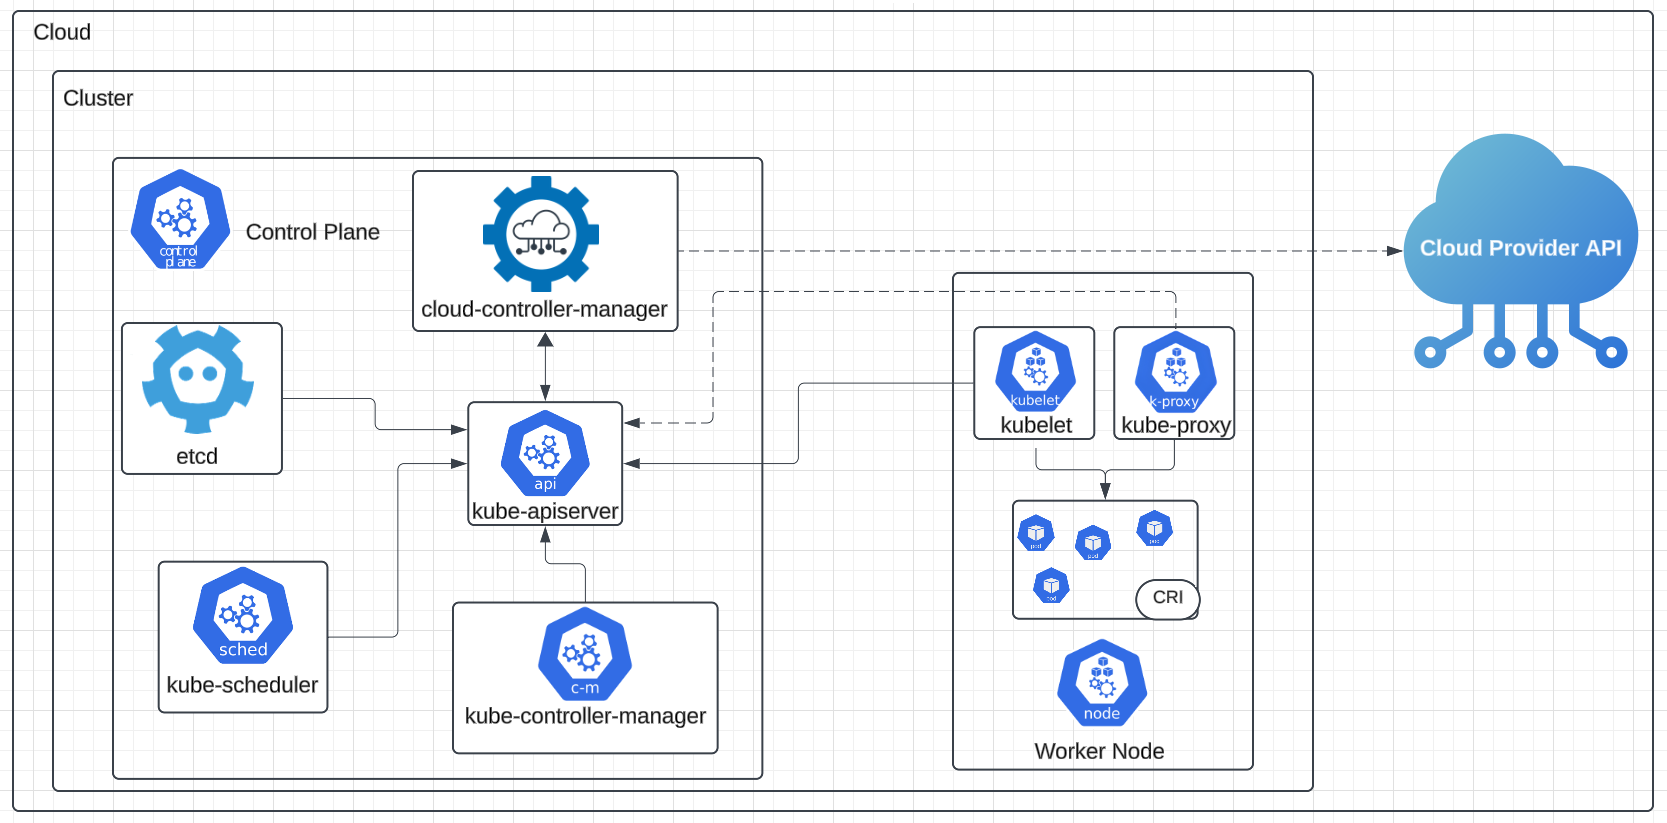
\includegraphics[width=1\columnwidth]{images/kubernetes-cluster-architecture.png}
    \caption{Kubernetes Cluster Architecture \cite{KubernetesArch}}
    \label{fig:k8s_arch}
\end{figure}

On figure~\ref{fig:k8s_arch} there is graphical representation of Kubernetes cluster. Not all of components shown in the figure are mandatory for Kubernetes to work correctly. At the control plane part, \textit{\nameref{sec:cloudControllerManager}} might not be mandatory, in on-premises configurations where interacting with cloud provider is not needed. On the right side of figure in node representation is \textit{\nameref{sec:kubeProxy}} component, which is not mandatory as some networking plugins can provide own implementation of proxy \cite{KubernetesArch}. This is an example of "Designed for extensibility", where Kubernetes can acquire 3rd-party features without changing its source code \cite{KubernetesDocs}.

% \begin{figure}[h!]
%     \centering
%     \includesvg[width=\textwidth]{}
%     \caption{An example image.}
%     \label{fig:example}
% \end{figure}



%---------------------------------------------------------------------------



\subsection{Control Plane}
\label{sec:k8s_cplane}

Control plane is like a brain in Kubernetes cluster. Interaction with cluster using kubectl tool to perform requests is handled by \textit{\nameref{sec:kubeApiServer}}. It is responsible for communication with worker nodes running pods, a smallest unit managed by K8s that has containers inside \cite{KubernetesArch}.

%---------------------------------------------------------------------------

\subsubsection{cloud-controller-manager}
\label{sec:cloudControllerManager}

This component allows Kubernetes cluster to interact with cloud provider's API. It is combined with kube-controller-manager as single binary and can be replicated. This is the only component that talks to the cloud provider, separating other components from direct communication with the cloud. When running without cloud envirnoment this component is absent \cite{KubernetesArch}.

%---------------------------------------------------------------------------

\subsubsection{etcd}
\label{sec:etcd}

Etcd is an open-source distributed key-value store service often used in distributed systems. It is responsible for maintaining both the current state and its previous version in its persistent memory \cite{KubernetesArch}\cite{Etcd}.

%---------------------------------------------------------------------------

\subsubsection{kube-apiserver}
\label{sec:kubeApiServer}

Exposes Kubernetes API to interact with a cluster. Takes responsibility for handling all requests from components and users. This is the component which answers cluster administrator requests sent by kubectl \cite{KubernetesArch}.

%---------------------------------------------------------------------------

\subsubsection{kube-controller-manager}
\label{sec:kubeControllerManager}

Component which runs controller processes. Its compiled binary consists of multiple controllers. Example controllers are \cite{KubernetesArch}:

\begin{itemize}
    \item Node controller -- observes worker nodes if are up and running
    \item Job controller -- responsible for batch execution jobs
    \item EndpointSlice controller -- connects services with pods
\end{itemize}

More controller names can be found in \href{https://github.com/kubernetes/kubernetes/blob/master/cmd/kube-controller-manager/names/controller_names.go}{Kubernetes source code}.

%---------------------------------------------------------------------------

\subsubsection{kube-scheduler}
\label{sec:kubeScheduler}

Takes care of pods which are not assigned to a worker node yet. kube-scheduler is looking for node that meets pod's scheduling requirements and fit a pod on that node. Such a node is called feasible node \cite{KubernetesScheduler}.

%---------------------------------------------------------------------------

\subsection{Nodes}
\label{sec:k8sNodes}
All of the below mentioned components run on every node in a cluster. 
%---------------------------------------------------------------------------

\subsubsection{Container runtime}
\label{sec:containerRuntime}

Node's key component, has ability to run, execute commands, manage and delete containers in efficient way \cite{KubernetesArch}. 

%---------------------------------------------------------------------------


\subsubsection{kube-proxy}
\label{sec:kubeProxy}

Create networking rules which allow to communicate with Pods from outside cluster. If available kube-proxy uses operating system packet filtering to create set of rules. It is also able to forward traffic by itself. This component is optional, can be replaced with a different one if the desired one implements key features. \cite{KubernetesArch}.

%---------------------------------------------------------------------------

\subsubsection{kubelet}
\label{sec:kubelet}

It is responsible for managing containers inside pod on its node. Uses Container Runtime Interface to communicate with containers \cite{KubernetesArch} \cite{KubernetesCRI}.

%---------------------------------------------------------------------------

\subsection{Objects}    
\label{sec:k8s_objects}

\subsubsection{Namespace}
\label{sec:namespace}

The purpose of namespace object is to isolate groups of resources like pods, deployments, services etc. in a cluster. It helps to organize cluster into virtual sub areas of working space. If \textit{\nameref{svc}} is created in some custom namespace <service-name>.<namespace-name>.svc.cluster.local DNS entry within cluster is created \cite{KubernetesNamespaces}.

\subsubsection{Pods}
\label{sec:pods}

Pods are the smallest deployable objects in Kubernetes. It contains one or more containers, which can communicate with each other using localhost interface. Since they share IP addresses, they cannot use the same ports. It is really useful, when our service consists of two apps which are coupled together. For example, there is a pod which has two containers, one responsible for compiling a code, the second one is creating cache entry from compiled object and uploads to some data storage. It makes more sense, as sharing data among containers in a pod is rather easier than on node between pods. Scaling is simpler than replicating one pod instead of two. Moreover, communication between apps happens using localhost, in scenario where there are two pods with one container, ClusterIP \textit{\nameref{svc}} is needed. However, the most common approach is to run one container per pod, where pod is just managing wrapper for containerized app. Also, rather than creating pod directly it is more common to use workload resource like \textit{\nameref{deployment}} \cite{KubernetesPods}. 


\subsubsection{ReplicaSet}
\label{replicaset}

Basically \textit{\nameref{replicaset}} consists of pod template and runs desired number of pods \cite{KubernetesReplicaSet}. 


\subsubsection{Deployment}
\label{deployment}

Deployment is a higher-level abstraction over \textit{\nameref{replicaset}}, that manages its lifecycle. It provides more features like rolling back an app, as it keeps history of configurations \cite{KubernetesDeployments}.

\subsubsection{DaemonSet}
\label{daemonset}

Running pods using DaemonSet guarantee that every node will have a copy of desired pod (if resource requirements are met etc.). It has the ability to automatically add or remove pods, if the number of nodes changes. The typical usage is creating monitoring pod on every node \cite{KubernetesDaemonSet}. 


\subsubsection{StatefulSet}
\label{statefulset}

StatefulSet unlike \textit{\nameref{deployment}} is stateful. It saves an identity of each pod and if e.g. some persistent storage is assigned to specific e.g. database pod and it dies, Kubernetes will recreate pod on the same node as it was previously \cite{KubernetesStatefulSet}.

\subsubsection{Job}
\label{job}

Runs pod that does one task and exists. Kubernetes will retry execution if pod fails specific number of tries set in its configuration \cite{KubernetesJobs}.

\subsubsection{CronJob}
\label{cronjob}
Behaviors like \textit{\nameref{job}} but is able to run regularly every given time for tasks like database backups or log rotation \cite{KubernetesCronJob}. 

\subsubsection{Service}
\label{svc}

Service exposes an application running inside a cluster by using an endpoint. As a pod is ephemeral resource and its address changes from time to time (e.g. when pod is recreated) it is better to create DNS name that resolves IP address. Moreover, the service will not advertise unhealthy pods. Usually, a service exposes one port per service, but for example web app might expose http and https ports. There are four types of services \cite{KubernetesService}. 


\begin{enumerate}
    \item ClusterIP -- makes one pod available to other inside cluster by exposing application using inter-cluster IP address. Although it's oriented to be accessible within the cluster, objects like \textit{\nameref{ingress}} or \textit{\nameref{gatewayapi}} can expose service to the outside.
    \item NodePort -- by default allocates port (from range 30000-32767) to publish service on every node's IP address. In this scenario every node on specified port acts like a proxy to deployed app.
    \item LoadBalancer -- Kubernetes does not provide load balancer by default and when creating such a service it interacts with cloud provider to create external service for traffic balancing. A load balancer can be installed inside cluster.
    \item ExternalName -- allows pods inside Kubernetes to access external service using defined name rather than using IP address 
\end{enumerate}

%---------------------------------------------------------------------------



\subsection{Cluster Networking}
\label{sec:k8s_networking}

Networking is the most important thing in Kubernetes, the whole point is to obtain reliable and robust communication among containers, pods, services, nodes and external systems in a cluster \cite{KubernetesClusterNetworking}. There are four types of network communication: \cite{KubernetesClusterNetworking}:

\begin{enumerate}
    \item container-to-container -- communicates by sharing network resources inside a pod
    \item Pod-to-Pod -- every pod can communicate with any other pod without the need to use NAT as every of them has its own IP address \cite{IBMKubernetesNetworking}.
    \item Pod-to-Service -- covered by service type ClusterIP, which provides inter-cluster IP address
    \item External-to-Service -- held by services type NodePort and Loadbalancer, which expose pod to the outside
\end{enumerate}
Kubernetes allocates IP addresses to nodes, services and pods \cite{KubernetesClusterNetworking}:
\begin{itemize}
    \item \textit{\nameref{sec:kubelet}} or \textit{\nameref{sec:cloudControllerManager}}, depending on local or cloud infrastructure allocates IP address for nodes
    \item \textit{\nameref{sec:kubeApiServer}} allocates IP address for services
    \item for allocation of IP address to pod is responsible networking plugin which is an implementation of \textit{\nameref{sec:cni}}
\end{itemize}


%---------------------------------------------------------------------------

\section{The Concept of Traffic Engineering in Kubernetes}
\label{sec:trafficConcept}

Traffic Engineering is a key concept in Kubernetes to provide production-ready, reliable and efficient network. In this section ingress and egress traffic will be explained.

%---------------------------------------------------------------------------

\subsection{Ingress Traffic Management}
\label{sec:ingressTrafficMngmnt}

\subsubsection{Ingress}
\label{ingress}

Ingress is an object that manages outside cluster access to services inside a cluster. It is a single point of entry to route traffic to specified pod based on configuration. This is only a higher abstract object that specifies routing rules in cluster. Real functionalities are provided by an \textit{\nameref{ingresscontroller}}. Nowadays the development of Ingress is frozen, Kubernetes authors pay attention to its successor a \textit{\nameref{gatewayapi}} \cite{KubernetesIngress}.

\subsubsection{Ingress Controller}
\label{ingresscontroller}

Ingress Controller fulfills an \textit{\nameref{ingress}} and starts serving an application which performs configured rules. Any implementation has its own features, but common functionalities are L4/L7 load balancing, host and path-based routing, SSL termination. This is the real application that runs in a pod. Ingress Controller have to be installed manually and is not part of Kubernetes, however the container orchestration tool developers maintain \href{https://github.com/kubernetes-sigs/aws-load-balancer-controller#readme}{AWS}, \href{https://github.com/kubernetes/ingress-gce/blob/master/README.md#readme}{GCE}, and \href{https://github.com/kubernetes/ingress-nginx/blob/main/README.md#readme}{nginx} ingress controllers \cite{KubernetesIngress}\cite{KubernetesIngressControllers}. 


\subsubsection{Gateway API}
\label{gatewayapi}

The functionalities of Gateway API are so wide, that the Kubernetes authors use term "project". The project mainly focuses on L4 and L7 routing in a cluster. It succeeds \textit{\nameref{ingress}}, Load Balancing and service mesh APIs. The Gateway API resource model is role-oriented \cite{KubernetesGatewayAPI}.

\begin{figure}[tbh]
    \centering
    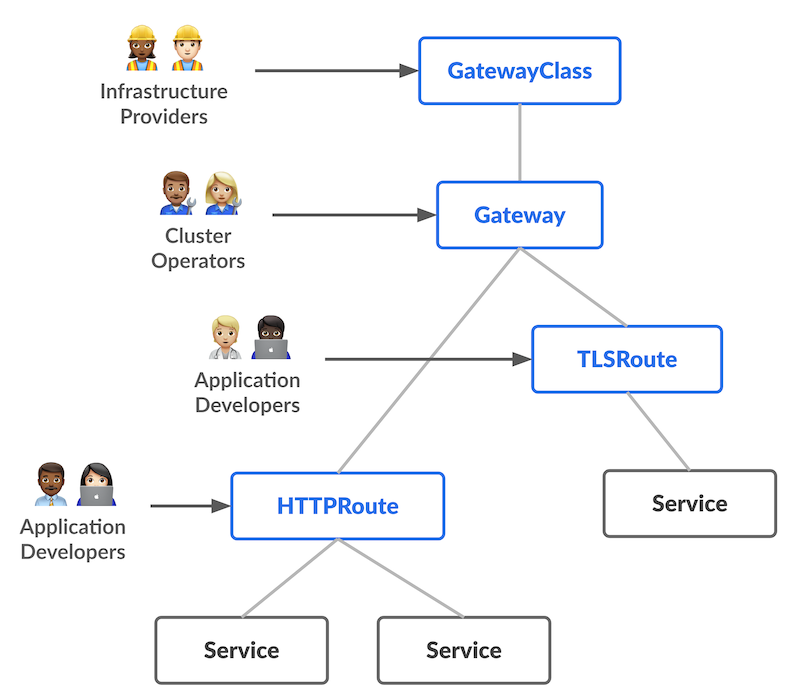
\includegraphics[width=0.7\columnwidth]{images/gateway-api-resource-model.png}
    \caption{Gateway API roles-oriented resource model \cite{KubernetesGatewayAPI}}
    \label{fig:gatewayApiResourceModel}
\end{figure}

The model focuses on 3 separate groups of people who interact with a cluster on different levels. 

On a top of figure~\ref{fig:gatewayApiResourceModel} there are infrastructure providers, who provide GatewayClass resource. They are responsible for the overall multiple clusters infrastructure, rather than ensuring developers can access pods correctly \cite{KubernetesGatewayAPI}. The Gateway API creators provide a clear overview of what GatewayClass is: "This resource represents a class of Gateways that can be instantiated.". It defines specific types of loadbalancing implementations and provides clear explenation of capabilities availabe in Kubernetes resource model. The functionality is similiar to \textit{\nameref{ingress}} \cite{KubernetesGatewayAPI} \cite{KubernetesGatewayClass}. There can be more than one GatewayClasss created. \cite{KubernetesGatewayAPI}. 


Cluster operators are in the middle of figure~\ref{fig:gatewayApiResourceModel}, they make sure that cluster meets requirements for several users. As maintainers define Gateway resource, some loadbalancing system is provisioned by GatewayClasss. Gateway resource defines specific instance which will handle incoming traffic. Allows to define specific protocol, port or allowed resources to route inbound traffic \cite{KubernetesGatewayAPI} \cite{KubernetesGateway}.

End users specified on Gateway API resource model on~\ref{fig:gatewayApiResourceModel} figure are application developers. They focus on serving applications to the clients by creating a resource named HTTPRoute. The resource defines HTTP routing from defined gateway to end API object like service. It is able to split traffic using "weight" as a key, which represents the percentage of the total traffic to be routed. GRPCRoute is simmiliar, but operates on different protocols. \cite{KubernetesGatewayAPI} \cite{KubernetesHTTPRoute}. 



Gateway API is not an API Gateway. An API Gateway in general is responsible for routing, load balancing, information exchange manipulation and much more depending on specific implementation. Gateway API is set of three resources mentioned earlier, which creates a role-oriented Kubernetes service networking model. Creators of Gateway API provide a clear explanation: "Most Gateway API implementations are API Gateways to some extent, but not all API Gateways are Gateway API implementations" \cite{KubernetesGatewayAPI}. 

%---------------------------------------------------------------------------

\subsection{Egress Traffic Management}
\label{sec:egressTrafficMngmnt}

Egress traffic refers to connections which leave cluster and are initiated inside by pods. In contrast to the Ingres object, in Kubernetes there is no Egress resource, outgoing traffic route logic is implemented by Container Network Interface plugin. The most common approach in managing egress traffic is to use Kubernetes Network Policies to deny all outgoing traffic and then allow only key connections. The limitation is that all external services need to be specified with IP address in policies. Any change in external resource's IP requires a change in policy configuration. If any pod is trying to access external service, source network access translation (SNAT) needs to be performed to map inter-cluster pod IP to externally routed nodes IP. When the response is accessing cluster, SNAT is performing translation in opposite way. Another key egress concept in Kubernetes is an egress gateway. This is a node which proxies outgoing traffic from a cluster, specified by provided configuration (e.g. by labeling pods, depends on CNI implementation). The important thing is that the internal pod's IP address is masqueraded into IP address of an egress gateway, outside peer does not see ephemeral IP of a pod. Egress gateway is also a CNI specific implemented resource. \cite{CalicoEgress} \cite{CiliumEgressGateway}. 


%---------------------------------------------------------------------------

\section{Container Network Interface (CNI)}
\label{sec:cni}
CNI is standardized by Cloud Native Computing Foundation set of API rules which defines container networking. Generally speaking, CNI is responsible for pod-to-pod communication, which includes assigning IP addresses, configuring network interface inside container and routing \cite{IBMKubernetesNetworking}. 



%---------------------------------------------------------------------------

\subsection{Overview of Selected CNI Plugins}
\label{sec:cni_overview}


\begin{table}[h!]
    \centering
    \caption{Comparison of Antrea and Cilium \cite{Antrea}\cite{CiliumBGP}\cite{CiliumEgressGateway}\cite{CiliumGatewayAPI}\cite{CiliumEncryption}.}
    \resizebox{\textwidth}{!}{%
    \begin{tabular}{|l|l|l|}
    \hline
    \textbf{Feature/Plugin}              & \textbf{Antrea}                                         & \textbf{Cilium}                                \\ \hline
    \textbf{Dataplane}            & Open vSwitch                                            & eBPF                                           \\ \hline
    \textbf{Encapsulation}        & VXLAN or Geneve                                         & VXLAN or Geneve                                \\ \hline
    \textbf{Encryption}           & IPsec or WireGuard tunnels                              & IPsec or WireGuard tunnels                     \\ \hline
    \textbf{Security}             & Extends Kubernetes Network Policies                     & Advanced security policies                     \\ \hline
    \textbf{Observability}        & Theia and Grafana for visualization                     & Hubble                                         \\ \hline
    \textbf{Purpose}              & Simplified Kubernetes networking management             & For large-scale cluters                        \\ \hline
    \textbf{Additional features}  & Network policies for non-Kubernetes nodes               & BGP to advertise network outside cluster       \\ \hline
    \textbf{Gateway API}          & No support                                              & Fully supports Gateway API                     \\ \hline
    \textbf{Egress Gateway}       & Basic egress gateway capabilities                       & Advanced egress gateway support                \\ \hline
    \end{tabular}}
    \label{tab:antrea_cilium}
\end{table}


Antrea is an open-source CNI plugin which is built on Open vSwitch \cite{Antrea}. OvS is a virtual switch with capability of handling traffic flow between virtual machines and containers \cite{OvS}. Antrea's main focus is L3/L4 networking and security services, such as network policies. The resource is responsible for managing traffic flow between pods. By default, every pod can communicate with any other pod, but network policies can specify if pod A is able to talk to pod B \cite{KubernetesNetworkPolicies}. Consider scenario with three pods, client, frontend and backend. There is no need to allow client communication directly with backend, so network policies allow traffic flow from client to frontend and direct communication with backend is not allowed \cite{CalicoNetworkPolicies}. 


Cilium, open-source CNI which uses eBPF (extended Barkeley Packer Filter) for packet processing, security and deep observability using Hubble \cite{CiliumOverview}. eBPF is a technology that allows running defined programs, with custom logic inside operating system kernel in privileged context without need of any kernel source code changes or loading modules. Lack of switching between kernel and user space, which reduces latency \cite{eBPF}. 

As seen on figure~\ref{fig:ebpf_routing}, the whole point of eBPF networking is skipping overhead that comes from iptables. Moreover, eBPF implements hash tables for storing routing policies, which time complexity is O(log n), compared to iptables array O(n). It makes clear that large-scale clusters will benefit from using eBPF \cite{IsovalentHash}. 

\begin{figure}[H]
    \centering
    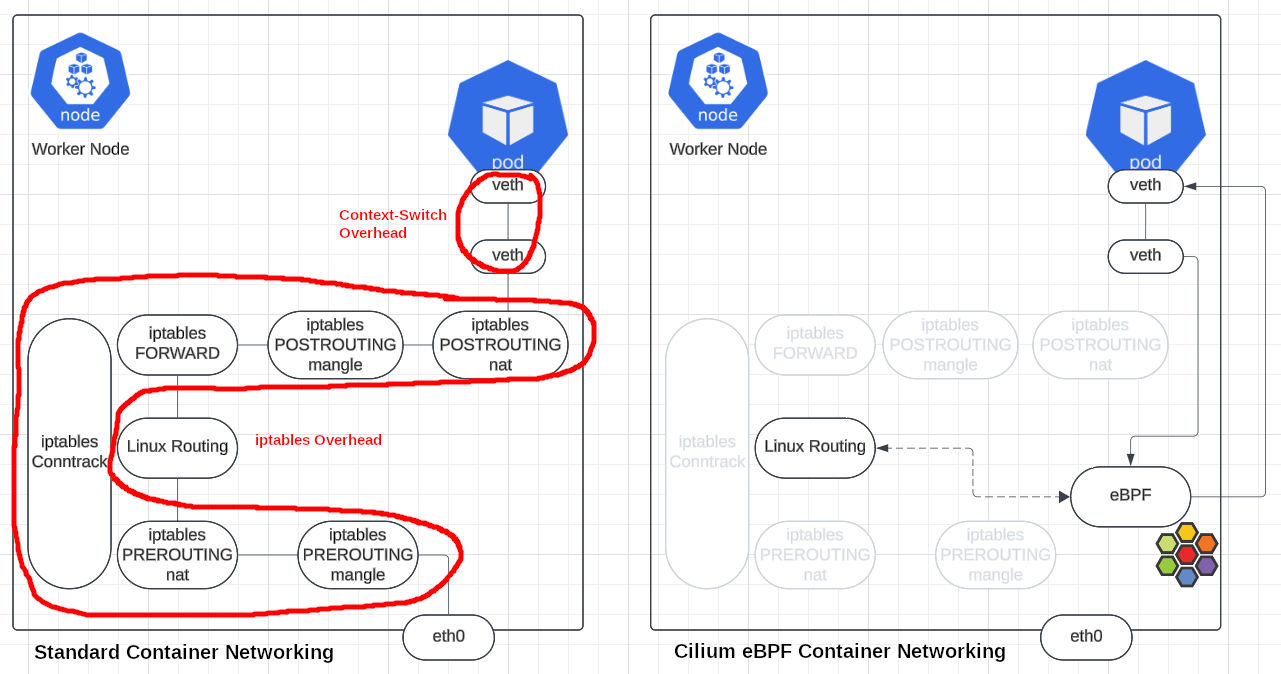
\includegraphics[width=0.9\columnwidth]{images/ebpf_hostrouting.png}
    \caption{Cilium eBPF host-routing \cite{CiliumCNIBenchmark}}
    \label{fig:ebpf_routing}
\end{figure}



%---------------------------------------------------------------------------

\section{Related Work}
\label{sec:realted_work}

As discussed in \cite{dakic2024performance} the performance of different CNIs can vary widely, some CNIs performing two to three times better than others, making it essential to choose the right plugin for a particular workload. Authors say, that developing automated methodology of CNI plugin evaluation is a key aspect, specifically in large High-Performance Computing (HPC) environments. This allows for reproducible and consistent tests across different configurations, reducing the overhead of manual testing. To achieve that, tools like Ansible can be helpful. They state that Linux Kernel or NIC can be a bottleneck in networking performance, so they extend maximum buffer size, scale TCP window, disable TCP Selective Acknowledgement, increase SYN Queue Size or enable Generic Receive offload. The paper shows results of comparison four CNI plugins, such as Antrea, Cilium, Calico, Flannel using TCP/UDP in base and with optimized system settings \cite{dakic2024performance}. 

In \cite{9153266} the authors measure CNI plugins for inter-host and intra-host communication using UDP and TCP protocols. They introduce the concept of CPU cycles per packet (CPP) to evaluate CNI efficiency. They measure CPP spent in each network component using the Linux perf tool. By measuring throughput, RTT, and latency, they compare how differ CNI plugins (flannel, weave, cilium, kube-router, calico) compared to its network models \cite{9153266}. 

Another paper \cite{9309003} of \cite{9153266} authors. Functionality, performance, and scalability are in main focus, the scale testbed up to 99 iperf client and 99 iperf server pod, mentioning that 100 pods are Kubernetes one node limit \cite{9309003}. 

The authors of \cite{10138542} state that in the coming years, fith generation mobile networks (5G) will deploy a significant part of their infrastructure in the cloud-native platforms, resulting in the creation of large-scale clusters. Such production environments containing thousands of pods require creating stable, reliable and efficient networks. They do not focus their attention on which CNI uses in this scenario, rather highlight such concepts as highly performant networking, security and observability. Authors state that the key to meet these expectation is eBPF (extended Barkeley Packet Filter) \cite{10138542}. 
